\subsection{اسلاید‌های دیجیتال}\label{subsec:اسلاید-های-دیجیتال}
همانطور که در قسمت قبل گفته شد، نمونه‌های تهیه‌شده از ناحیه‌های مشکوک بیمار از غده تیروئید، توسط دستگاه‌هایی اسکن می‌شوند و به صورت تصاویری دیجیتال در می‌آیند که برای کامپیوتر‌های قابل خواندن هستند.
قبل از اینکه این نمونه‌ها توسط دستگاه اسکن شوند ممکن است فرآیندی روی نمونه‌ها انجام شود تا سلول‌ها در زیر میکروسکپ و یا در تصویر دیجیتال به خود رنگ بگیرند.
این کار به متخصصین کمک می‌کنند تا سلول‌ها را راحت تر از دیگر مواد داخل نمونه تشخیص دهند و این باعث افزایش دقت تشخیص می‌شود.
به همین دلیل اسلاید‌های تهیه‌شده به این روش، ممکن است رنگ‌های مختلفی به خود بگیرند.


نمونه‌ای از این اسلاید‌ها در شکل ~\autoref{fig:sampleWSIscan} آمده است که از مجموع‌داده \cite{ncigdc} برداشته شده که اندازه‌ی تصویر اصلی آن برابر با
 $114240\times30077$
 پیکسل است.

\begin{figure}
    \begin{center}
        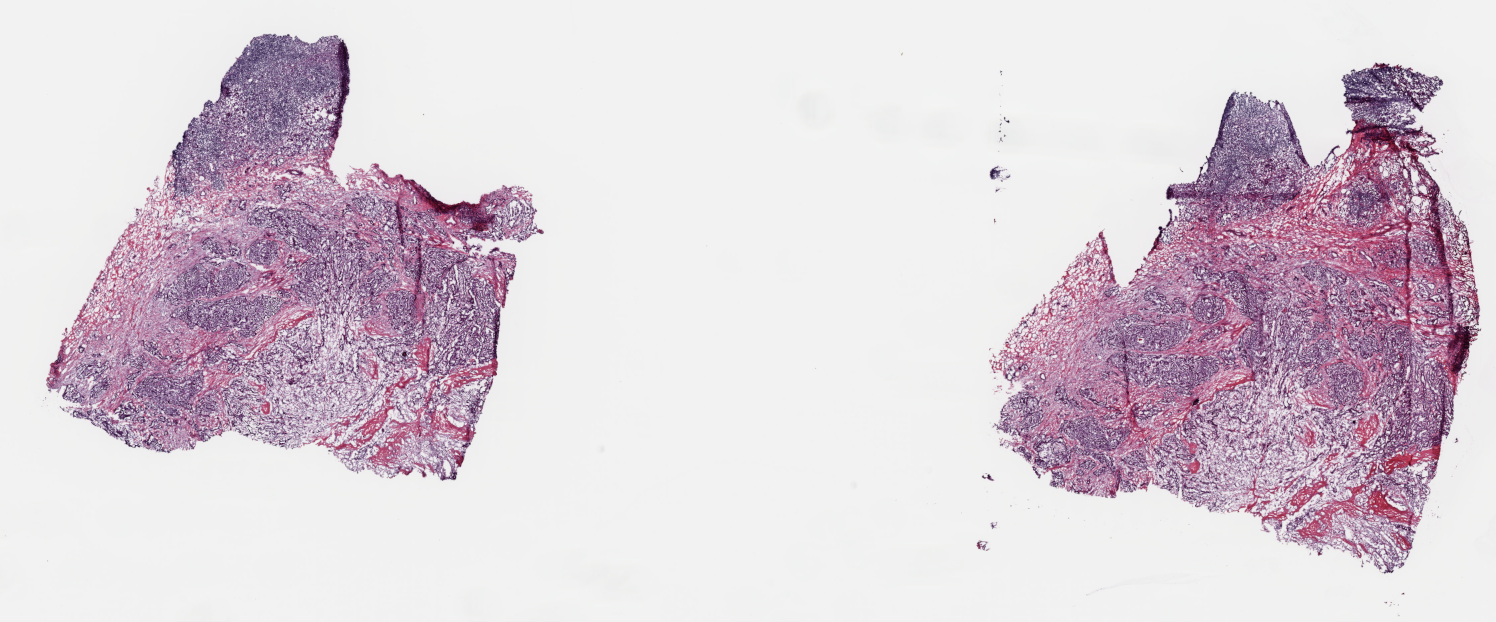
\includegraphics[width=\linewidth]{figs/basic_concepts/subs/Sample Slide From NCI.PNG}
    \end{center}
    \caption{نمونه اسلاید اسکن‌شده از غده تیروئید}
    \label{fig:sampleWSIscan}
\end{figure}
عکس‌های دیگر از این نمونه‌ها که توسط روش‌های مختلف رنگ آمیزی شده‌اند نیز در شکل ~\autoref{fig:samplecoloringfrompapsociety} آمده است.
منبع این شش تصویر نیز مجموع‌داده \cite{papsocietyiamgeatlas} است.
\begin{figure}
	\begin{center}
		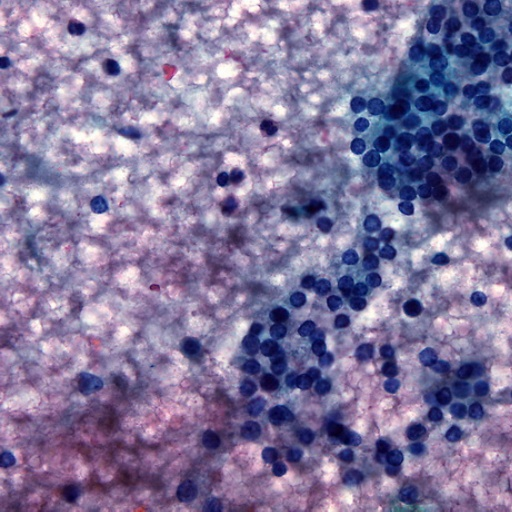
\includegraphics[width=0.3\linewidth]{figs/basic_concepts/subs/different_coloring/-2107274412359028693-3.jpeg}
		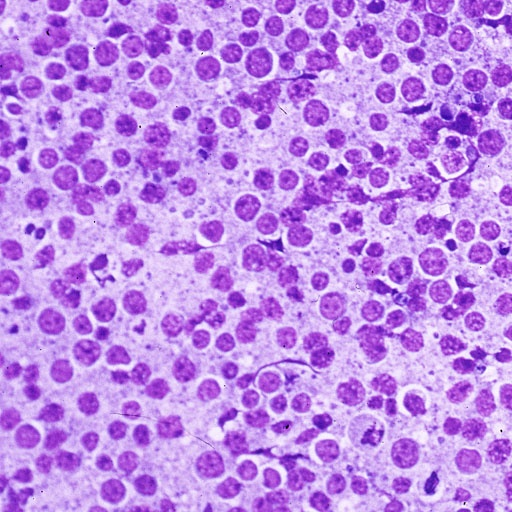
\includegraphics[width=0.3\linewidth]{figs/basic_concepts/subs/different_coloring/-519123361907272548-1.jpeg}
		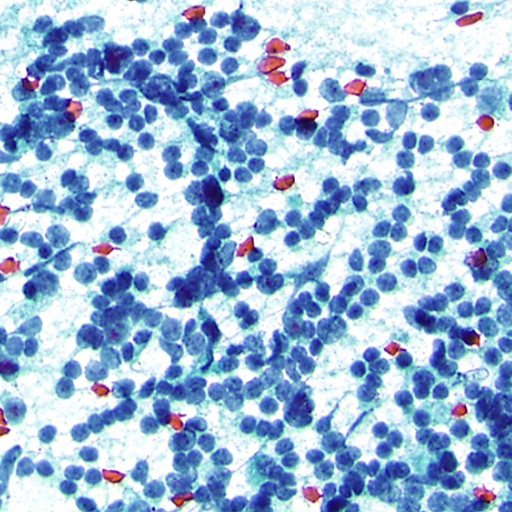
\includegraphics[width=0.3\linewidth]{figs/basic_concepts/subs/different_coloring/-951104570143882402-2.jpeg}		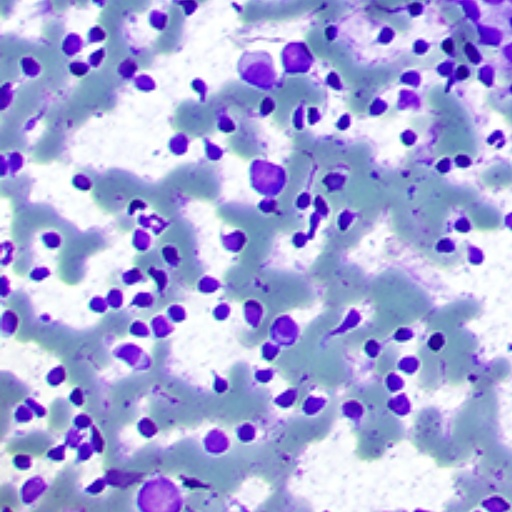
\includegraphics[width=0.3\linewidth]{figs/basic_concepts/subs/different_coloring/2689566490603340021-23.jpeg}	
		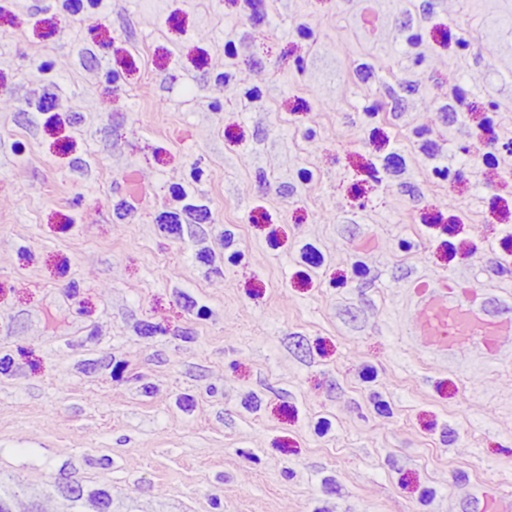
\includegraphics[width=0.3\linewidth]{figs/basic_concepts/subs/different_coloring/-454345013748557057-2.jpeg}	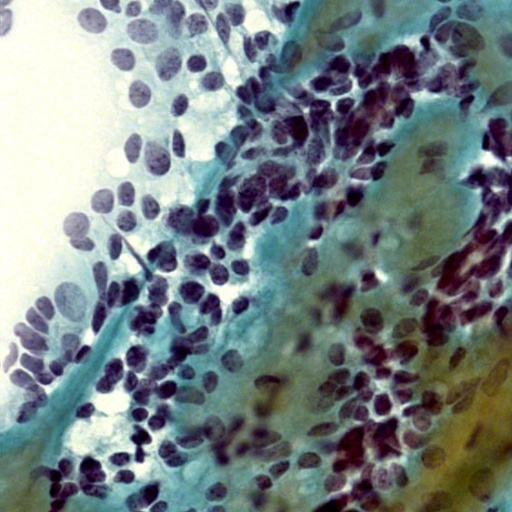
\includegraphics[width=0.3\linewidth]{figs/basic_concepts/subs/different_coloring/2970953228795442512-2.jpeg}
	\end{center}
	\caption{نمونه اسلاید اسکن‌شده از غده تیروئید با رنگ امیزی‌های متفاوت}
	\label{fig:samplecoloringfrompapsociety}
\end{figure}
این اسلاید‌ها معمولا ابعاد بسیار بزرگی دارند و ممکن است تا بزرگنمایی 40 برابر را پشتیبانی کنند.
به همین دلیل ممکن است حجمی بین چند مگابایت تا چند گیگابایت را به خود بگیرند.
